\documentclass{standalone}

\usepackage{amsmath, amssymb, amsthm}
\usepackage{tikz}

\usetikzlibrary{shapes.geometric, arrows}

\tikzstyle{block} = [draw, fill=white, rectangle,
    minimum width=3cm, minimum height=0.5cm]

\begin{document}
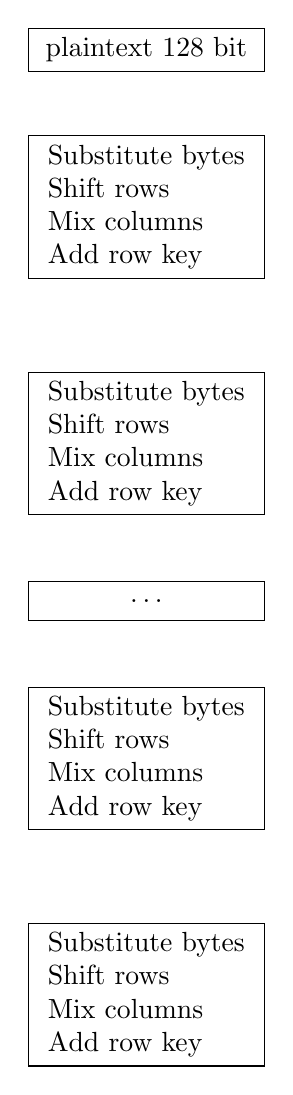
\begin{tikzpicture}[node distance=2cm]
    \node [block] (ptx) {plaintext 128 bit};
    \node [block, below of=ptx, align=justify] (r1) {Substitute bytes \\ Shift rows \\ Mix columns \\ Add row key};
    \node [block, below of=r1, align=justify, node distance=3cm] (r2) {Substitute bytes \\ Shift rows \\ Mix columns \\ Add row key};

    \node [block, below of=r2] (tmp) {$\ldots$};

    \node [block, below of=tmp, align=justify] (r9) {Substitute bytes \\ Shift rows \\ Mix columns \\ Add row key};
    \node [block, below of=r9, align=justify, node distance=3cm] (r10) {Substitute bytes \\ Shift rows \\ Mix columns \\ Add row key};

\end{tikzpicture}

\end{document}